
%\todo{Start here. 4 pages each and 2 pages discussion. Target 20 pages.}

%msection{Generating Software Diversification for WebAssembly}

\Wasm programs are produced ahead of time through a process that begins with the source code and moves through the compiler, ultimately resulting in a \Wasm program. 
Software Diversification can be achieved at any of these stages. 
Diversifying at the source code stage, however, is not practical due to the necessity of creating a distinct diversifier for each language compatible with \Wasm. 
In contrast, focusing on the compiler stage presents a viable option, especially considering that 70\% of \Wasm binaries are created using LLVM-based compilers, as noted by Hilbig et al. \cite{Hilbig2021AnES}. 
Furthermore, implementing diversification at the \Wasm program stage stands as the most generic strategy, applicable to any \Wasm program in the wild. 
Therefore, this thesis focuses to the exploration of diversification strategies at the compiler and \Wasm program stages, employing two main approaches: compiler-based and binary-based.


\begin{figure}[h]
	\centering
	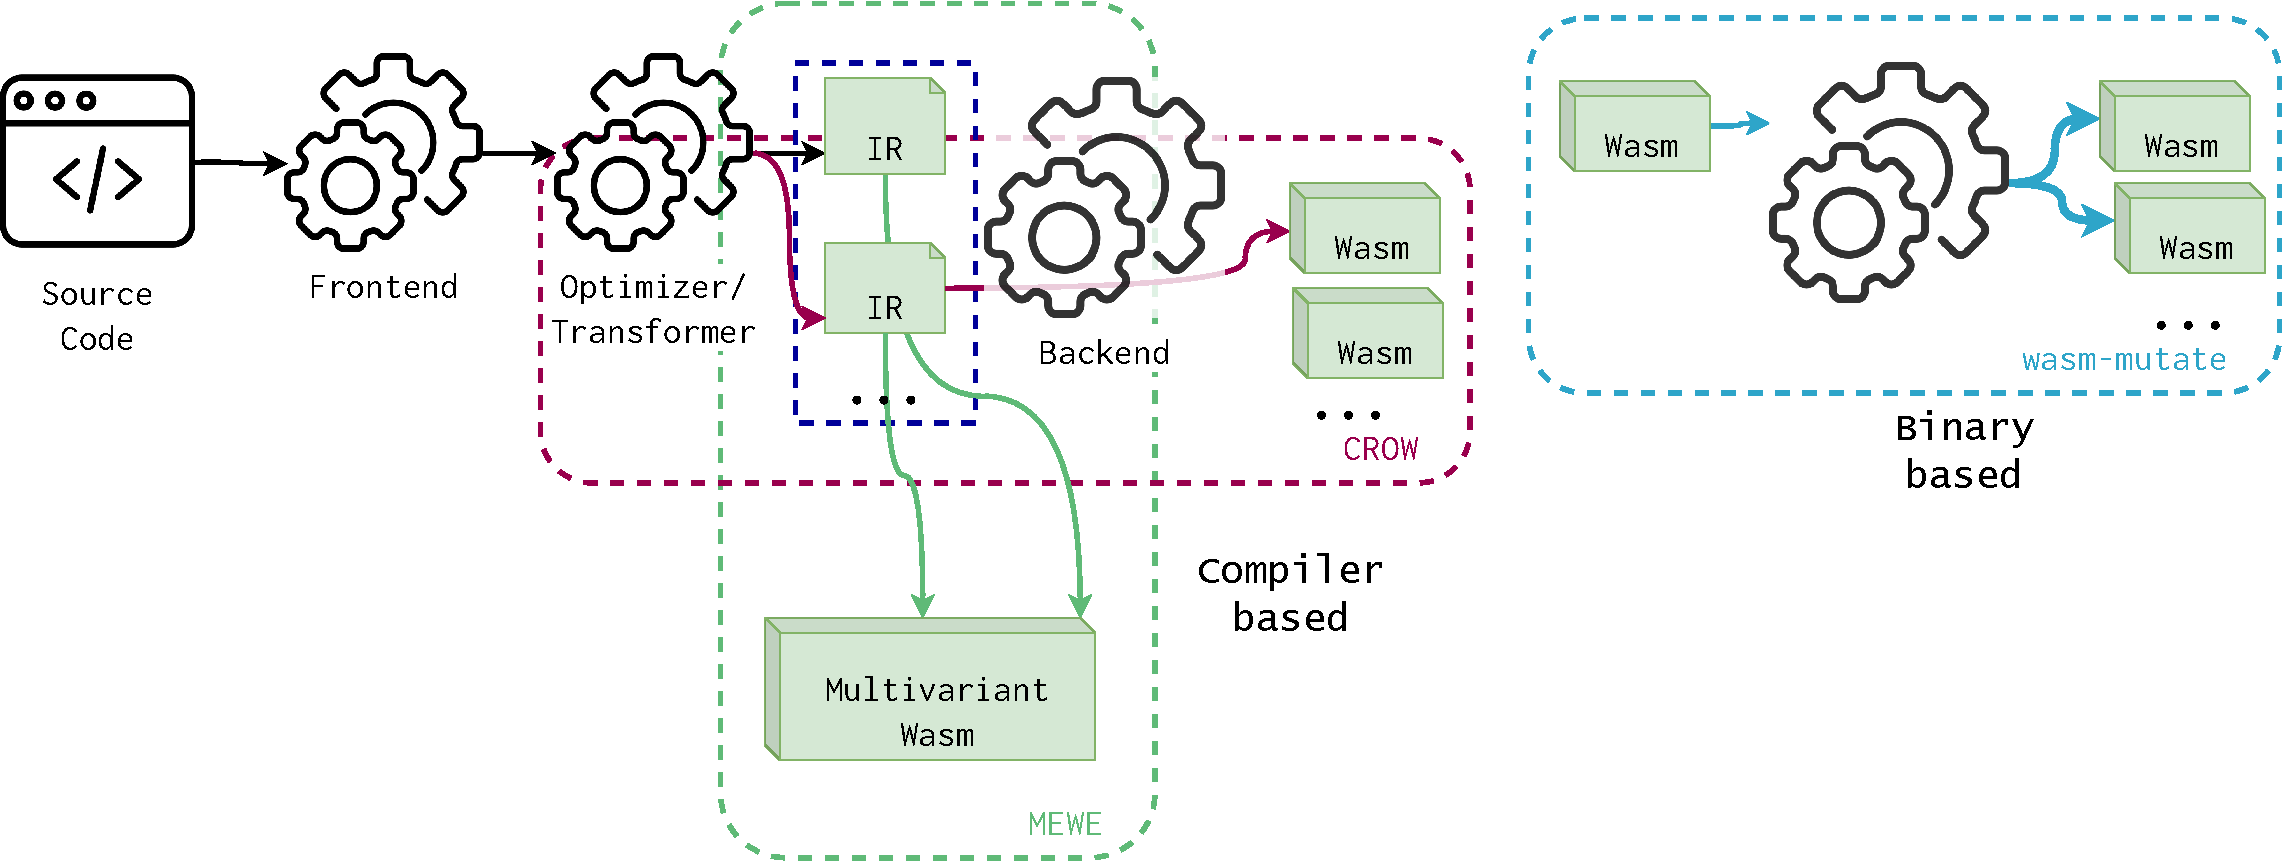
\includegraphics[width=1.0\textwidth]{figures/landscape.pdf}
	\caption{Approach landscape.}
	\label{fig:approach_landscape}
\end{figure}

% Compiler based approaches
Our compiler-based strategies are depicted in red and green in \autoref{fig:approach_landscape}. 
This approach introduces a diversifier component in the LLVM pipeline, generating LLVM IR variants and producing artificial software diversity for \wasm. 
This strategy encompasses two tools: CROW \cite{CROW}, which creates \wasm program variants, and MEWE \cite{MEWE}, which merges these variants to foster multivariant execution for \wasm.
In contrast, the binary-based strategy, illustrated in blue in \autoref{fig:approach_landscape}, offers diversification for any \Wasm program. 
wasm-mutate \cite{wasm-mutate} generates a pool of \Wasm program variants through rewriting rules upon an e-graph \cite{e-graph} data structure, eliminating the need for compiler tuning.
This dissertation contributes to the field of Software Diversification for \Wasm, presenting three main technical contributions: CROW, MEWE, and wasm-mutate, which will be elaborated upon in the subsequent sections.

